%!TEX root = ../main.tex

\graphicspath{{./figures/chapter4/}}


\chapter{Spatial feature engineering} \label{ch:chapter4}
\minitoc
\newpage

In this chapter we present and discuss different approaches to analyze \ac{RNA} localization patterns.
They require to quantify and measure indicators from fluorescent images.
To do so, we use a coordinate representation of cells, merging results from the detection~\ref{ch:chapter2} and segmentation~\ref{ch:chapter3} chapters.

We first present this representation, obtained with methods implemented in \emph{bigfish.multitask}.
In the second and third parts of this chapter we then present two different methods to compute spatial features.
We can manually design localization features or we can learn them, training a gradient-based pipeline on a pretext task.

The hand-crafted features are already implemented in \emph{bigfish.classification}.
The learned features section was mainly developed with the paper:

\begin{center}
	\color{green}
	Future paper to be released (ECCV workshop or arxiv)
\end{center}

\section{From images to coordinates} \label{sec:image_coordinates}

We mainly base our analysis on the coordinate representation of cells as illustrated in figure~\ref{fig:cell_extracted_0}.
We exploit outcomes from detection and segmentation stages.
More precisely, we extract and identify for each individual cell coordinates of detected objects and segmentation masks.
As a reminder, current implementation in \emph{bigfish} allows a 2D or 3D detection, but only a 2D segmentation.
However, any external methods could be used, as long as output format fits.

\begin{figure}[h]
    \centering
    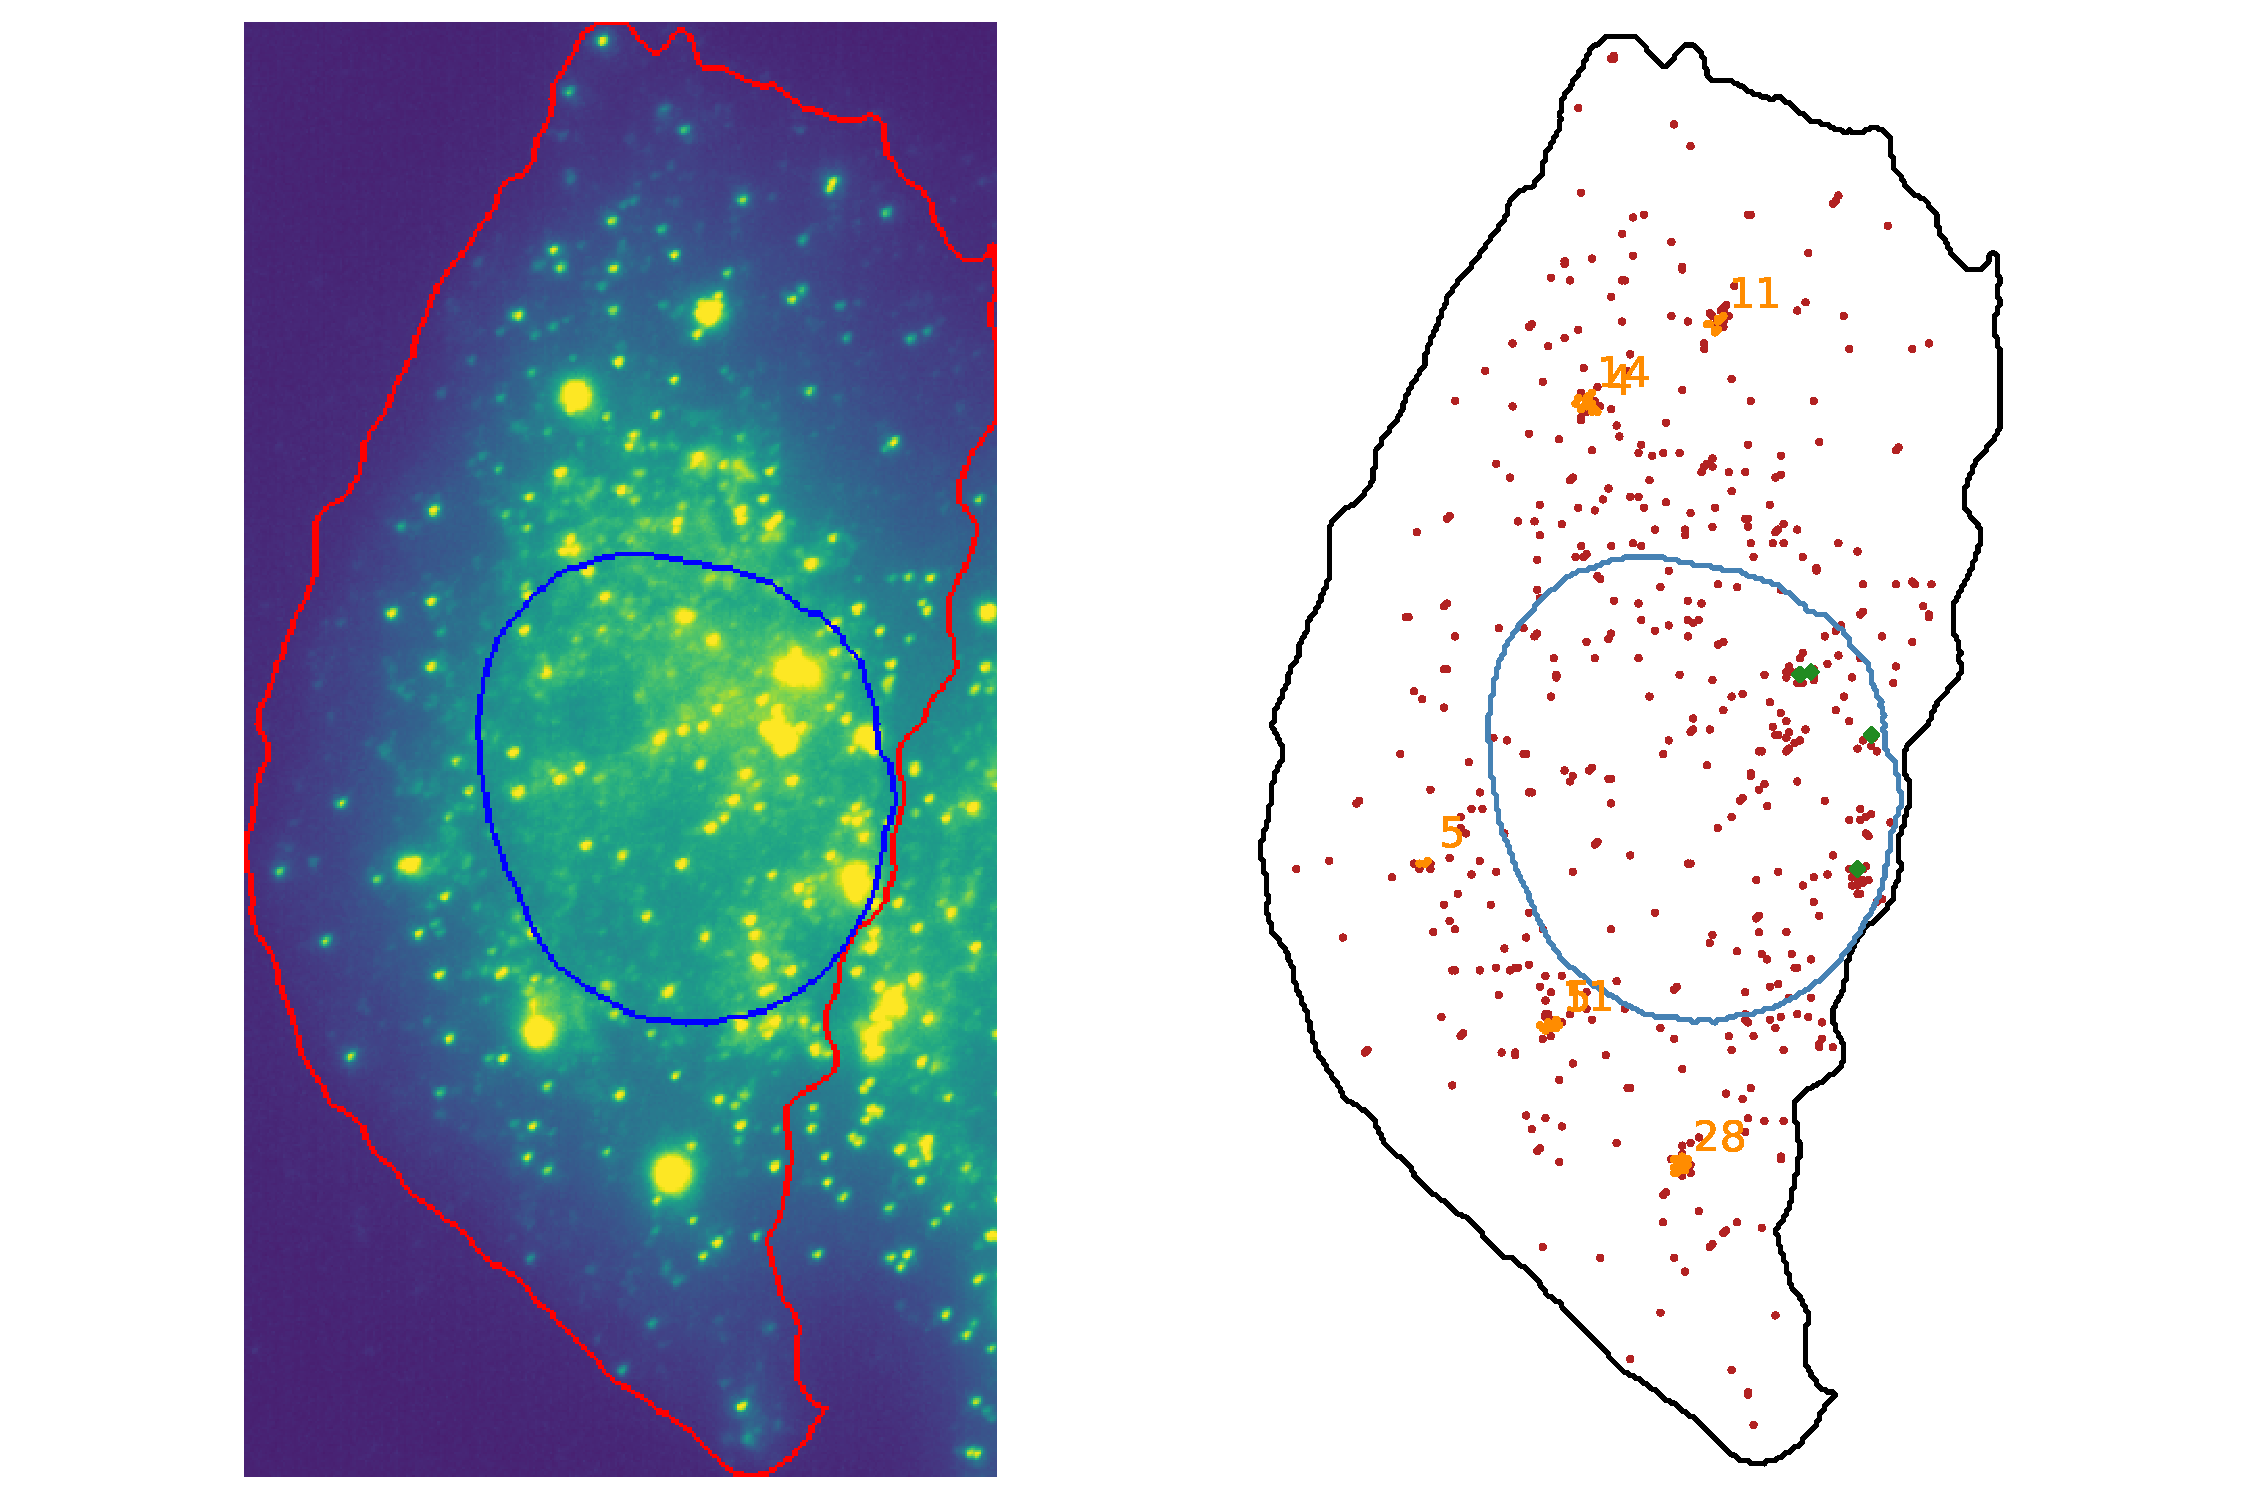
\includegraphics[width=1\textwidth]{figures/chapter4/cell_extracted_0}
    \caption{Original image (left) and coordinate representation (right)}
    \label{fig:cell_extracted_0}
\end{figure}

\paragraph{Detected object labelling}

In addition to detection and segmentation refinement, the possibility to merge results from both stages is highly valuable.
We can discriminate individual objects according to their localization in the cell.
A user might want to label a detected object if it locates within a segmented surface or not.
For example, some studies require to remove transcription sites before further analysis~\cite{CHOUAIB_2020}, or on the contrary to focus on them.
User could define a \ac{RNA} cluster inside nucleus as a transcription site, as opposed to the ones detected outside nucleus.
More generally, any detected object could be assigned to a specific cellular compartments, depending on the fluorescent labels available in the study.\\

% reference paper using transcription site only

\begin{minipage}{0.9\textwidth}
\begin{lstlisting}[language=Python]
import bigfish.multistack as multistack

# discriminate foci and transcription sites
spots_no_ts, foci, ts = multistack.remove_transcription_site(
	rna=spots,
	clusters=clusters,
	nuc_mask=nuc_label,
	ndim=3)
\end{lstlisting}
\end{minipage}

\paragraph{Cell extraction}

To extract and summarize our \ac{FISH} results at the single cell level, the only requirement is a segmentation mask of the cell.
At least, user needs to perform instance segmentation to be able to identify individual cells.
Additional results are optional, but they greatly improve the quality of the information assigned to each cell.
Detected \ac{RNA} and cluster (or anything else detected) can be assigned to individual cells.
Nuclei segmentation masks make us able to delimitate nuclear membrane and define transcription sites or any nucleus-related object.
We can also crop input images around the identified cells, for every available channels.

In figure~\ref{fig:cell_extracted_0} we can observe a cropped \ac{smFISH} image on the left, with cell and nuclear membranes in red and blue respectively.
On the right, these membranes are also visible (in black and blue respectively), in addition with \ac{RNA} spots (in red), \ac{RNA} clusters (in orange, with the estimated number of \ac{RNA} clustered) and transcription sites (in green).
With such \emph{extraction} we lose pixel-wise information like intensity values or image texture.
We also deeply rely on detection and segmentation performances to return meaningful coordinates.
Nonetheless, coordinate representation is a sparse and more natural representation for \ac{mRNA} localization pattern classification.
Indeed \ac{mRNA} molecules can be viewed as single point objects distributed in a 3D space.
Microscopic images with fluorescent labels are here the only medium we have to measure and approximate their localization.

Eventually we propose optional criteria to identify individual cells and refine the outcome.
First, we can ensure that only one nucleus is assigned to each cell.
Second, we can remove cropped cells at the border of the \ac{FoV}.
Their segmentation is incomplete and might bias final results.
Third, extracted cells can be filtered out according to the number of detected objects (especially the number of \ac{RNA}).
By censoring empty cells, we remove potential outliers, detection or segmentation failures and therefore help a subsequent statistical analysis.\\

\begin{minipage}{0.9\textwidth}
\begin{lstlisting}[language=Python]
import bigfish.multistack as multistack

# extract cell-level results
fov_results = multistack.extract_cell(
    cell_label=cell_label,
    ndim=3,
    nuc_label=nuc_label,
    rna_coord=spots_no_ts,
    others_coord={"foci": foci, "transcription_site": ts},
    image=image_contrasted,
    others_image={"dapi": nuc_mip, "smfish": smfish_mip})
\end{lstlisting}
\end{minipage}

\paragraph{Statistical description}

At this stage we can already compute standard, but useful statistics for every cells.
We measure cell and nucleus areas, but also \ac{RNA} distribution, inside and outside nucleus.
With cluster coordinates, estimation of cluster size is available, as well as proportion of clustered \ac{RNA}.
The \ac{RNA} proportion in specific cellular compartments are also noteworthy.
Such indicators are already relevant to quantify or validate meaningful biological insights.
For example, a recent study~\cite{cochard_rna_2022} use \emph{bigfish} to estimate \ac{RNA} recruitment in bioengineered condensates (segmented from a \ac{GFP} channel).\\

\begin{minipage}{0.9\textwidth}
\begin{lstlisting}[language=Python]
import bigfish.multistack as multistack

# compute cell-level statistics
df = multistack.summarize_extraction_results(fov_results, ndim=3)
\end{lstlisting}
\end{minipage}

\section{Hand-crafted localization features} \label{sec:hand_features}

We now present the first approach to analyze \ac{RNA} localization patterns in depth: we manually design spatial features.

\subsection{Related work} \label{subsec:related_work_hand_features}

% reference classical fish analysis (battich + stoegger + aubin)
% reference dypfish
% reference spatial statistics (carolina whelbi)

%~\cite{savulescu_interrogating_2021}
%~\cite{samacoits_computational_2018}
%~\cite{stoeger_computer_2015}
%~\cite{mcquin_cellprofiler_2018}
%~\cite{held_cellcognition_2010}
%~\cite{berg_ilastik_2019}
%~\cite{shariff_automated_2010}
%~\cite{laux_interactive_2020}
%~\cite{ljosa_introduction_2009}
%~\cite{battich_image-based_2013}
%~\cite{battich_control_2015}

%Feature engineering
%Aubin designed features from the cloud point representation
%of the cell in order to discriminate the different localization patterns. He
%gathered more than 20 features in a tabular format
%(one row per cell), ready to feed a machine learning model.
%A first set of features is based on the euclidean distance. We compute the distance between each
%mRNAs and the centroid of the cell, the centroid of the nucleus, the cell border and
%the nucleus border. Averages and quantiles are then computed from these distances and finally normalized.
%A second set of features involved the Ripley K-function. It quantifies the aggregation or dispersion of mRNAs:
%K(r)=1∑n Npi(r) (7) nλ
%i=1
%with r the distance range, Npi (r) the number of mRNAs in a circle of radius r centered
%on the ith mRNA and λ the total density of mRNAs in the cell (the total number of mRNAs
%normalized by the cell area). Several features are returned from this function like the
%maximum values, the Spearman correlation with the radius r, etc... Such features are
%useful to discriminate foci patterns. A corrected version of the function is actually
%used, less sensitive to boundary effects (mRNAs close to a border have a limited neighbourhood).
%A third set of features is based on morphological opening (an erosion followed by a dilation).
%Applying openings with different sizes, we remove cell’s extensions. We can count the mRNAs
%we loose and compute their proportion with the total number of mRNAs. The idea is to detect
%RNA localization in cell extensions.
%A final group of features concern the proportion of mRNAs inside the nucleus, a dispersion
%and a polarization index.
%1 Ripley: maximum
%2 Ripley: max gradient [0,max]
%3 Ripley: min gradient [max,end]
%4 Ripley: value at mid-point between center and boundary
%5 Ripley: Spearman correlation between Ripley and radius
%6 Ripley: radius of max value
%7 Polarization index
%8 Dispersion index
%9–12 Morph opening–enrichment ratio: 15, 30, 45, 60 pixels
%13 Cell height: Spearman correlation with ZmRNA
%14 Cell height: R2 with ZmRNA
%15 Cell membrane: distance – mean
%16-19 Distance membrane: quantile 5%, 10%, 20%, 50%
%20 Nucleus: distance – mean
%21 Cell centroid: distance – mean
%22 Nucleus centroid: distance – mean
%23 Ratio: mRNAs inside nucleus/outside nucleus

\subsection{Expert features} \label{subsec:expert_features}

A large part of hand-crafted features we implemented in \emph{bigfish.classification} were initially designed for our own studies~\cite{CHOUAIB_2020,safieddine_choreography_2021,pichon_kinesin_2021}.
These features capture more specific information about \ac{RNA} localization, beyond surface areas (\emph{cell\_area} and \emph{nuc\_area}) or expression levels (\emph{nb\_rna}).

\paragraph{Distance features}

We first reuse and adapt some distance features already implemented in the first FISH-quant version and presented in a recent paper~\cite{samacoits_computational_2018}.
Distances from cell or nuclear membranes are computed in 2D as we only use 2D segmentation results so far.
However, such features could be easily extended with 3D segmentation masks.

We compute the average distance between detected \ac{RNA}s and cell membrane \emph{index\_mean\_distance\_cell} such that:

\begin{equation}
	{\displaystyle \operatorname{index\_mean\_distance\_cell} = \frac{\overline{d_{cell}(x_i, y_i)}}{\lambda_{cell}}}
\end{equation}

\noindent
With $d_{cell}(x_i, y_i)$ the euclidean distance to the cell membrane for the rna $i$ and $\lambda_{cell}$ the expected average distance under uniform \ac{RNA} distribution.
A previous study~\cite{battich_control_2015} used the square root of cell area to normalize its distance features.
However, as noticed by~\cite{samacoits_computational_2018}, it does not take into account a potential heterogeneity in term of cell morphology.
For this reason we approximate $\lambda_{cell}$ as the average value of the 2D distance map from the cell membrane.
Similarly, we compute the normalized average distance of \ac{RNA}s to the nucleus: \emph{index\_mean\_distance\_nuc}.
Alternative computation with the median function is available for these two features too.

Unlike the first FISH-quant version, we do not compute distances to cell or nucleus centroids, nor quantiles of the \ac{RNA} distance distribution.
These features might appear redundant to quantify distance information.

\paragraph{Morphological features}

A second set of features is related to the localization of \ac{RNA} in specific cell compartments.
We already count the number of transcripts detected inside the nucleus.
More precisely, proportion of \ac{RNA}s inside the nucleus (\emph{proportion\_rna\_in\_nuc}) is a good enough indicator to identify intranuclear pattern.

\begin{figure}[h]
    \centering
    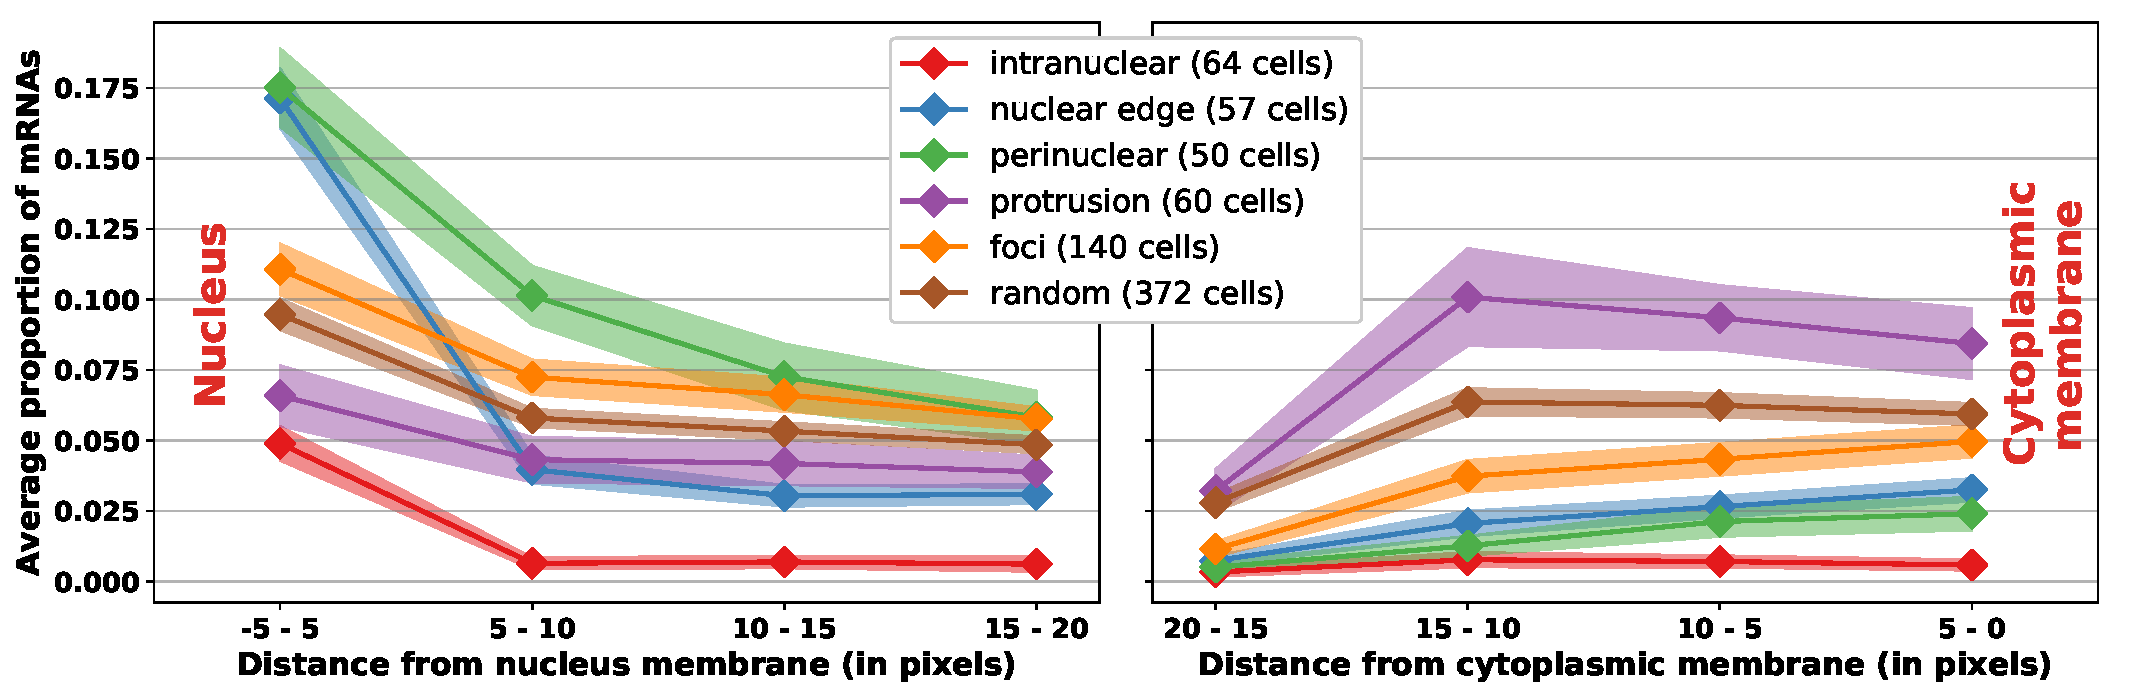
\includegraphics[width=1\textwidth]{figures/chapter4/plot_topography}
    \caption{Proportion of \ac{mRNA} at various distances from cell and nuclear membranes}
    \label{fig:features_topography}
\end{figure}

Still we can go further to partition cell regions.
We define a list of features to measure the distribution of \ac{RNA}s within different cell regions.
Regions of interest are delimited with concentric circles from cell or nuclear membranes, with an interval distance of 500nm each.
More precisely, area between 0 and 3000nm from the cell membrane is divided in six concentric regions.
In each region we compute \ac{RNA} proportion (\emph{proportion\_rna\_cell\_radius\_1000\_1500} for the proportion between 1000nm and 1500nm from the cell membrane) or we count the number of \ac{RNA}s we detect, normalized by the expected number of \ac{RNA}s under random distribution (\emph{index\_rna\_cell\_radius\_1000\_1500}).
We define 5 more regions around the nuclear membrane between 500nm and 3000nm.
Lastly, a larger region is defined along the nuclear membrane, including detected \ac{RNA}s inside or outside the nucleus, but within 500nm from its membrane.
Likewise, proportion (\emph{proportion\_rna\_nuc\_radius\_500\_1000}) and \ac{RNA} count (\emph{index\_rna\_nuc\_radius\_500\_1000}) are computed for all regions.
When we manually annotate real cells and identify different localization pattern we measure how discriminative these features can be.
In figure~\ref{fig:features_topography} we can observe average \ac{RNA} proportion for the different regions we described.
The 95\% confidence interval is also reported in the plot.
Logically, nuclear edge and perinuclear patterns present a higher proportion of \ac{RNA} along the nuclear membrane.
On the opposite, cells with a protrusion pattern have a higher \ac{RNA} density along the cell membrane.

We focus on a last relevant region in a cell: protrusions.
To design cell extension related features, we first need to define such extension.
Like~\cite{samacoits_computational_2018} we define this region as the lost area after applying a morphological opening (an erosion followed by a dilation) to the cell mask.
For this operation we use a disk with 3000nm radius as a structuring element.
We then compute the proportion of \ac{RNA} (\emph{proportion\_rna\_protrusion}) or the normalized \ac{RNA} count (\emph{index\_rna\_protrusion}) in protrusion.

\paragraph{Dispersion features}

We implement three features described and tested in a recent paper~\cite{stueland_rdi_2019} to quantify \ac{RNA} polarization and dispersion within the cell.

The polarization index (\emph{index\_polarization}) is computed by comparing \ac{RNA} point cloud and cell centroids:

\begin{equation}
	{\displaystyle \operatorname{index\_polarization} = \frac{\sqrt{(x_{rna} - x_{cell})^2 + (y_{rna} - y_{cell})^2}}{Rg_{cell}}}
\end{equation}

\noindent
With $(x_{rna}, y_{rna})$ the coordinates of the \ac{RNA} centroid and $(x_{cell}, y_{cell})$ the coordinates of the cell centroid.
The radius of gyration $Rg_{cell}$ normalizes the index for different cell sizes.
It is defined as the root-mean-squared distance between every cell pixels and the cell centroid.
The higher, the more polarized \ac{RNA}s are.

The dispersion index (\emph{index\_dispersion}) measures the dispersion of the \ac{RNA} point cloud.
In addition to the extracted coordinates, its computation also implies pixel intensities from the original \ac{smFISH} image:

\begin{equation}
	{\displaystyle \operatorname{index\_dispersion} = \frac{\frac{\sum_{i} r_i^2 I_i}{\sum_{i} I_i}}{\frac{\sum_{j} r_j^2 I_j}{\sum_{j} I_j}}}
\end{equation}

\noindent
With $r_i$ and $r_j$ the euclidean distance of \ac{RNA} $i$ and cell pixel $j$ to the \ac{RNA} centroid respectively, $I_i$ the pixel intensity of \ac{RNA} $i$ and $I_j$ the pixel intensity of cell pixel $j$.
Pixel intensity of transcripts distant from the \ac{RNA} centroid are overweighted.
As the index is normalized considering every pixels $j$ from the cell mask, it tends to 1 when \ac{RNA} point cloud is uniformly distributed.
A diffuse point cloud has a value greater than 1.
On the opposite, if \ac{RNA}s are concentrated anywhere in the cell, index value is lower than 1.

The peripheral distribution index (\emph{index\_peripheral\_distribution}) measures how close the \ac{RNA}s localize to the cell periphery.
Its computation is similar to the dispersion index, but the \ac{RNA} centroid is replaced by the nucleus one in the equation.
A completely dispersed point cloud still has a value of 1, but it increases if \ac{RNA}s move toward the cell periphery, with a concentrated or diffused pattern.
Again, an aggregation of transcripts around the nucleus centroid (often close to the cell centroid too) decreases index value.

\paragraph{Centrosomal features}

\begin{wrapfigure}{R}{0.40\textwidth}
  \begin{center}
    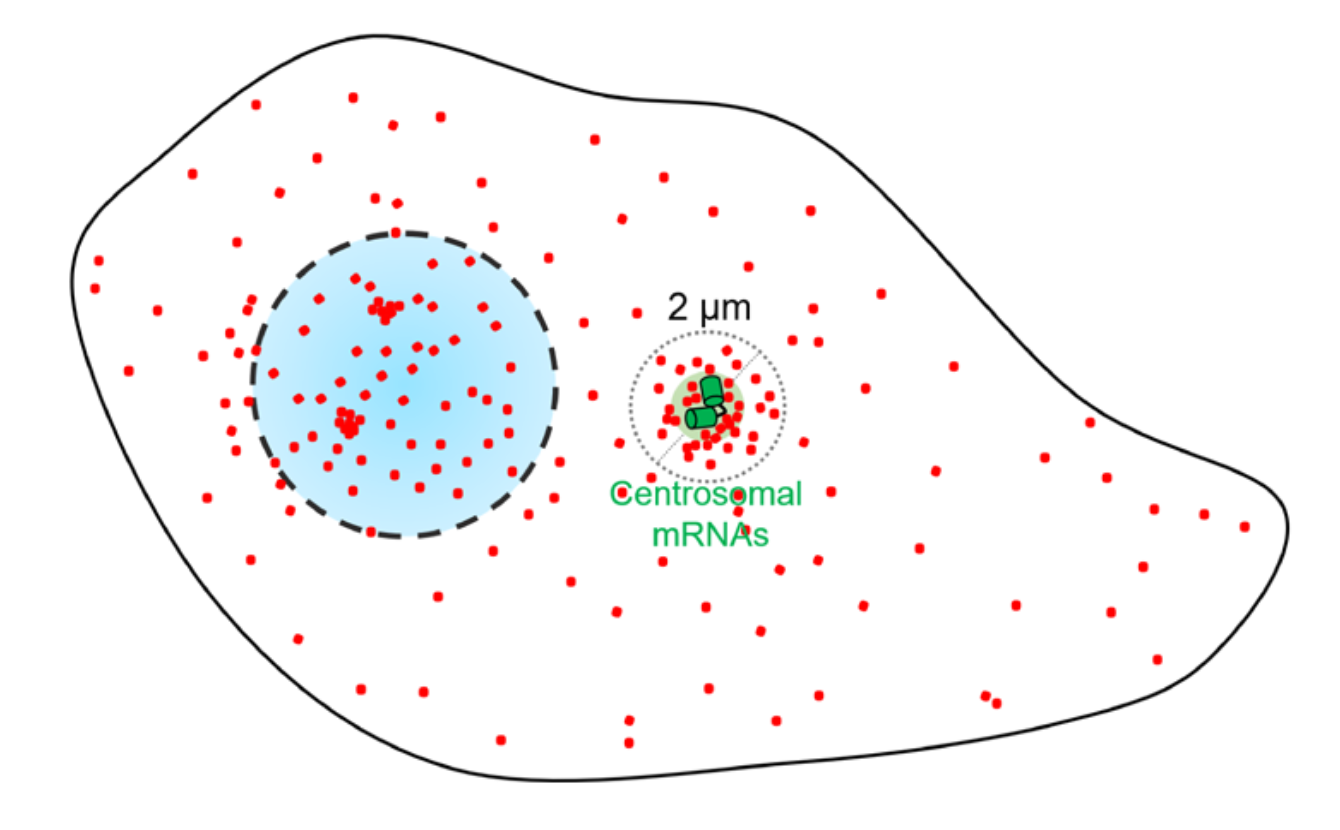
\includegraphics[width=0.33\textwidth]{figures/chapter4/centrosomal_features}
  \end{center}
  \caption{Centrosomal \ac{RNA}s (from~\cite{safieddine_choreography_2021})}
  \label{fig:centrosome_features}
\end{wrapfigure}

If we detect additional object and extract new coordinates besides individual and clustered \ac{RNA}s, more specific features can be designed.
For example, these objects can be cell organelles labelled during the experimentation and targeted for a study.
We design such features with the centrosomes to further study \ac{RNA} localization related to the \ac{MTOC}.

A first obvious feature is the average (or median) distance between \ac{RNA}s and the closest detected centrosomes (up to two centrosomes can be detected in the cell): \emph{index\_mean\_distance\_centrosome}.
Similarly to the distance features we compute with the cell or nuclear membranes, we compute the expected distance under uniform \ac{RNA} distribution for normalization.

A second set of features consists in delimiting an area around each centrome to be considered as centrosome neighbors.
In our case we manually choose a radius of 2000nm around centrosomes to define such areas, as illustrated in figure~\ref{fig:centrosome_features}.
We can then compute the normalized \ac{RNA} count (\emph{index\_rna\_centrosome}) or the \ac{RNA} proportion (\emph{proportion\_rna\_centrosome}) in these regions.

Lastly, we derived a feature from the dispersion index described above.
We define a centrosomal dispersion index to quantify \ac{RNA} dispersion around centrosomes: \emph{index\_centrosome\_dispersion}.
We design it like the dispersion index, but instead of \ac{RNA} centroid, we use the closest centrosome coordinates to compute the euclidean distance.
The lower, the closer \ac{RNA}s localized to the centrosomes.

\paragraph{Cluster features}

Concerning cluster localization patterns, we observed than our clustering method (see subsection~\ref{subsec:dense_decomposition}) already captures good enough information.
More specifically, number of detected clusters (\emph{nb\_foci}) or \ac{RNA} proportion inside these clusters (\emph{proportion\_rna\_in\_foci}) are relevant features to identify transcripts with a tendency for clustering.
As a consequence, and unlike~\cite{samacoits_computational_2018}, we do not implement diverse features based on the famous Ripley's K-function.
This would require tuning a lot more parameters than just reusing the detected number of clusters.

\begin{minipage}{0.9\textwidth}
\begin{lstlisting}[language=Python]
import bigfish.classification as classification

# compute features
features, features_names = classification.compute_features(
    cell_mask=cell_mask,  # individual cell mask
	nuc_mask=nuc_mask,  # individual nucleus mask
	ndim=3,
	rna_coord=rna_coord,
    smfish=smfish,
	voxel_size_yx=103,  # in nanometer
    foci_coord=foci_coord,
    compute_distance=True,
    compute_intranuclear=True,
    compute_protrusion=True,
    compute_dispersion=True,
    compute_topography=True,
    compute_foci=True,
    compute_area=True,
    return_names=True)
\end{lstlisting}
\end{minipage}

\section{Learned localization features} \label{sec:learned_features}

% intro subsections

\subsection{Related work} \label{subsec:related_work_learned_features}

% references neural network to build features
% 3-4 papers cnn features in image
% 3-4 papers cnn features in bioimage
% 3-4 papers cnn features with protein localization
% Bouilohol

% 1-2 paper review (deep laerning with bioimage)
% paper isbi + reference appendix
% 1-2 paper review (deep learning with point cloud)

% transition from cnn to pointcloud (pb localization with cnn // protein localization == texture classification)

%~\cite{dubois_deep_2019}

% pointnet
% dgcnn
% pointtransformer
% pointmlp

% general review shape classification with point cloud (kernel, curve, pointcnn, voxel3D)

% ML and DL (pointnet) to classify caveolae clusters and non-caveolae clusters
%%~\cite{khater_caveolae_2019}
%% Specifically, we are generating abalanced dataset of 1000 blobs of isotropic
%% point clouds and 1000 blobs of non-isotropic point clouds. The isotropic
%% class of blobs mimicking the caveolae (positive class) and the non-isotropic
%% class mimicking the non-caveolae (negative class). The non-isotropic class of
%% blobs are more planar structures, while the isotropic class are more spherical
%% structures.
%
%% Caveolae are plasma membrane invaginations whose formation requires caveolin-1 (Cav1),
%% the adaptor protein polymerase I,and the transcript release factor (PTRF orCAVIN1).
%% Caveolae have an important role incell functioning, signaling, and disease. Inthe
%% absence ofCAVIN1/PTRF, Cav1 forms non-caveolarmembrane domains called scaffolds.
%% Inthis work, we train machine learning models toautomatically distinguish between
%% caveolae and scaffolds from single molecule localization microscopy (SMLM) data
%% The first uses arandom forest classifier applied to28 hand-crafted/designed features
%% (expert features), the second uses aconvolutional neural net (CNN) applied toaprojection
%% ofthe point clouds onto three planes, and the third uses aPointNet model, a recent
%% development that can directly take point clouds as its input.

\subsection{Pretext task: simulated pattern classification} \label{subsec:simulation_localization}

% plot simulations
% explain simulations

\begin{figure}[h]
    \centering
    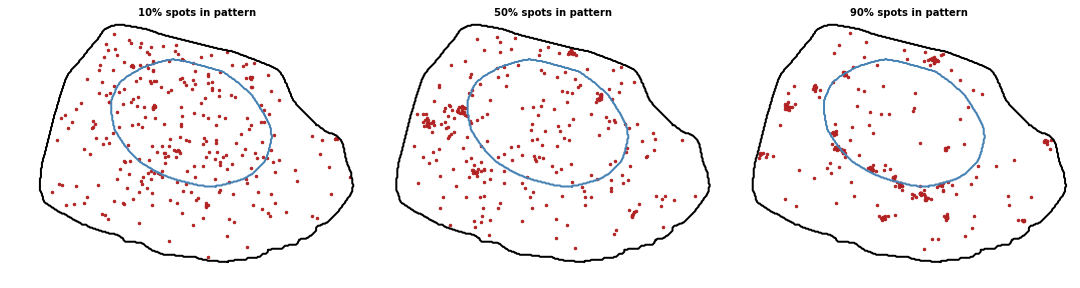
\includegraphics[width=1\textwidth]{figures/chapter4/foci_panel}
    \caption{Foci pattern simulations}
    \label{fig:foci_panel}
\end{figure}

\begin{figure}[h]
    \centering
    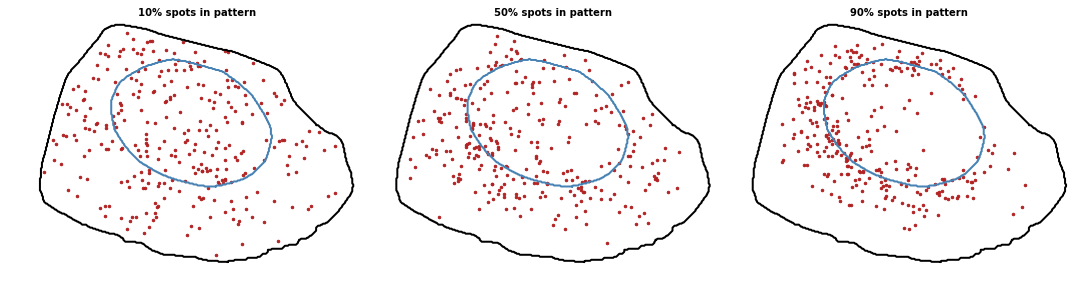
\includegraphics[width=1\textwidth]{figures/chapter4/perinuclear_panel}
    \caption{Perinuclear pattern simulations}
    \label{fig:perinuclear_panel}
\end{figure}

\begin{minipage}{0.9\textwidth}
\begin{lstlisting}[language=Python]
import simfish as sim

# load template dataset
path_template_directory = load_extract_template(path_output)

# localization pattern simulation
instance_coord = sim.simulate_localization_pattern(
	path_template_directory,
	n_spots=150,
	pattern="intranuclear",
	proportion_pattern=0.6)
\end{lstlisting}
\end{minipage}

\subsection{PointFISH} \label{subsec:pointfish}

% architecture description
% plot architecture
% training process
% results simulation
% plot matrix confusion simulation
% ablation studies (table)

\begin{figure}[h]
    \centering
    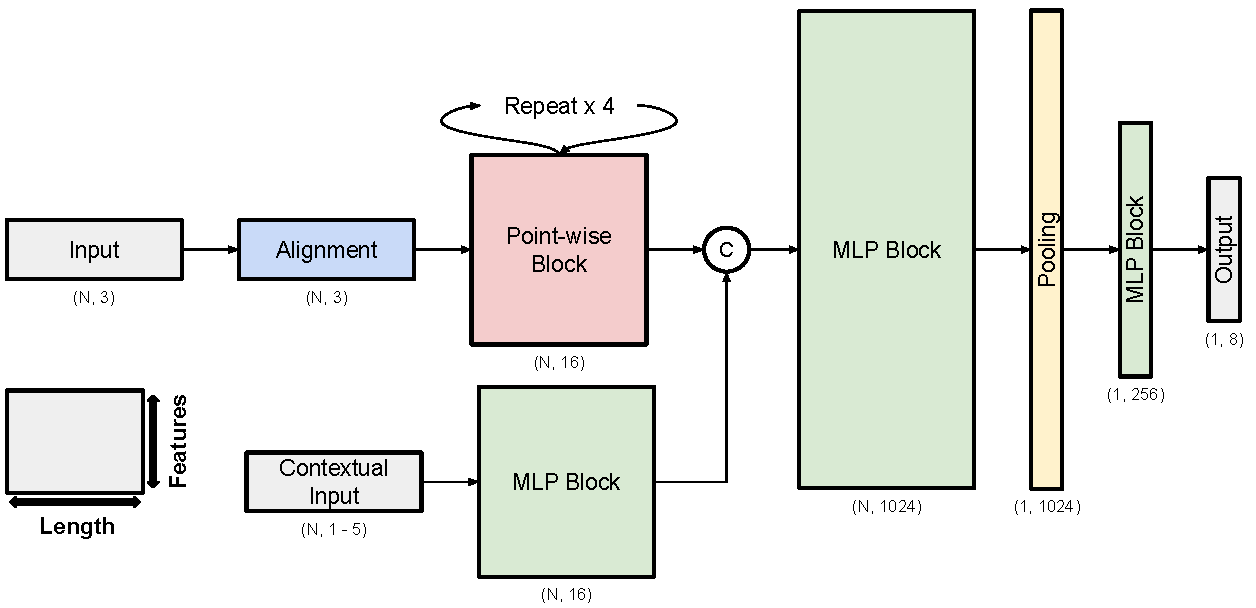
\includegraphics[width=1\textwidth]{figures/chapter4/PointFISH_architecture}
    \caption{PointFISH architecture template}
    \label{fig:PointFISH_architecture}
\end{figure}

\begin{figure}[h]
    \centering
    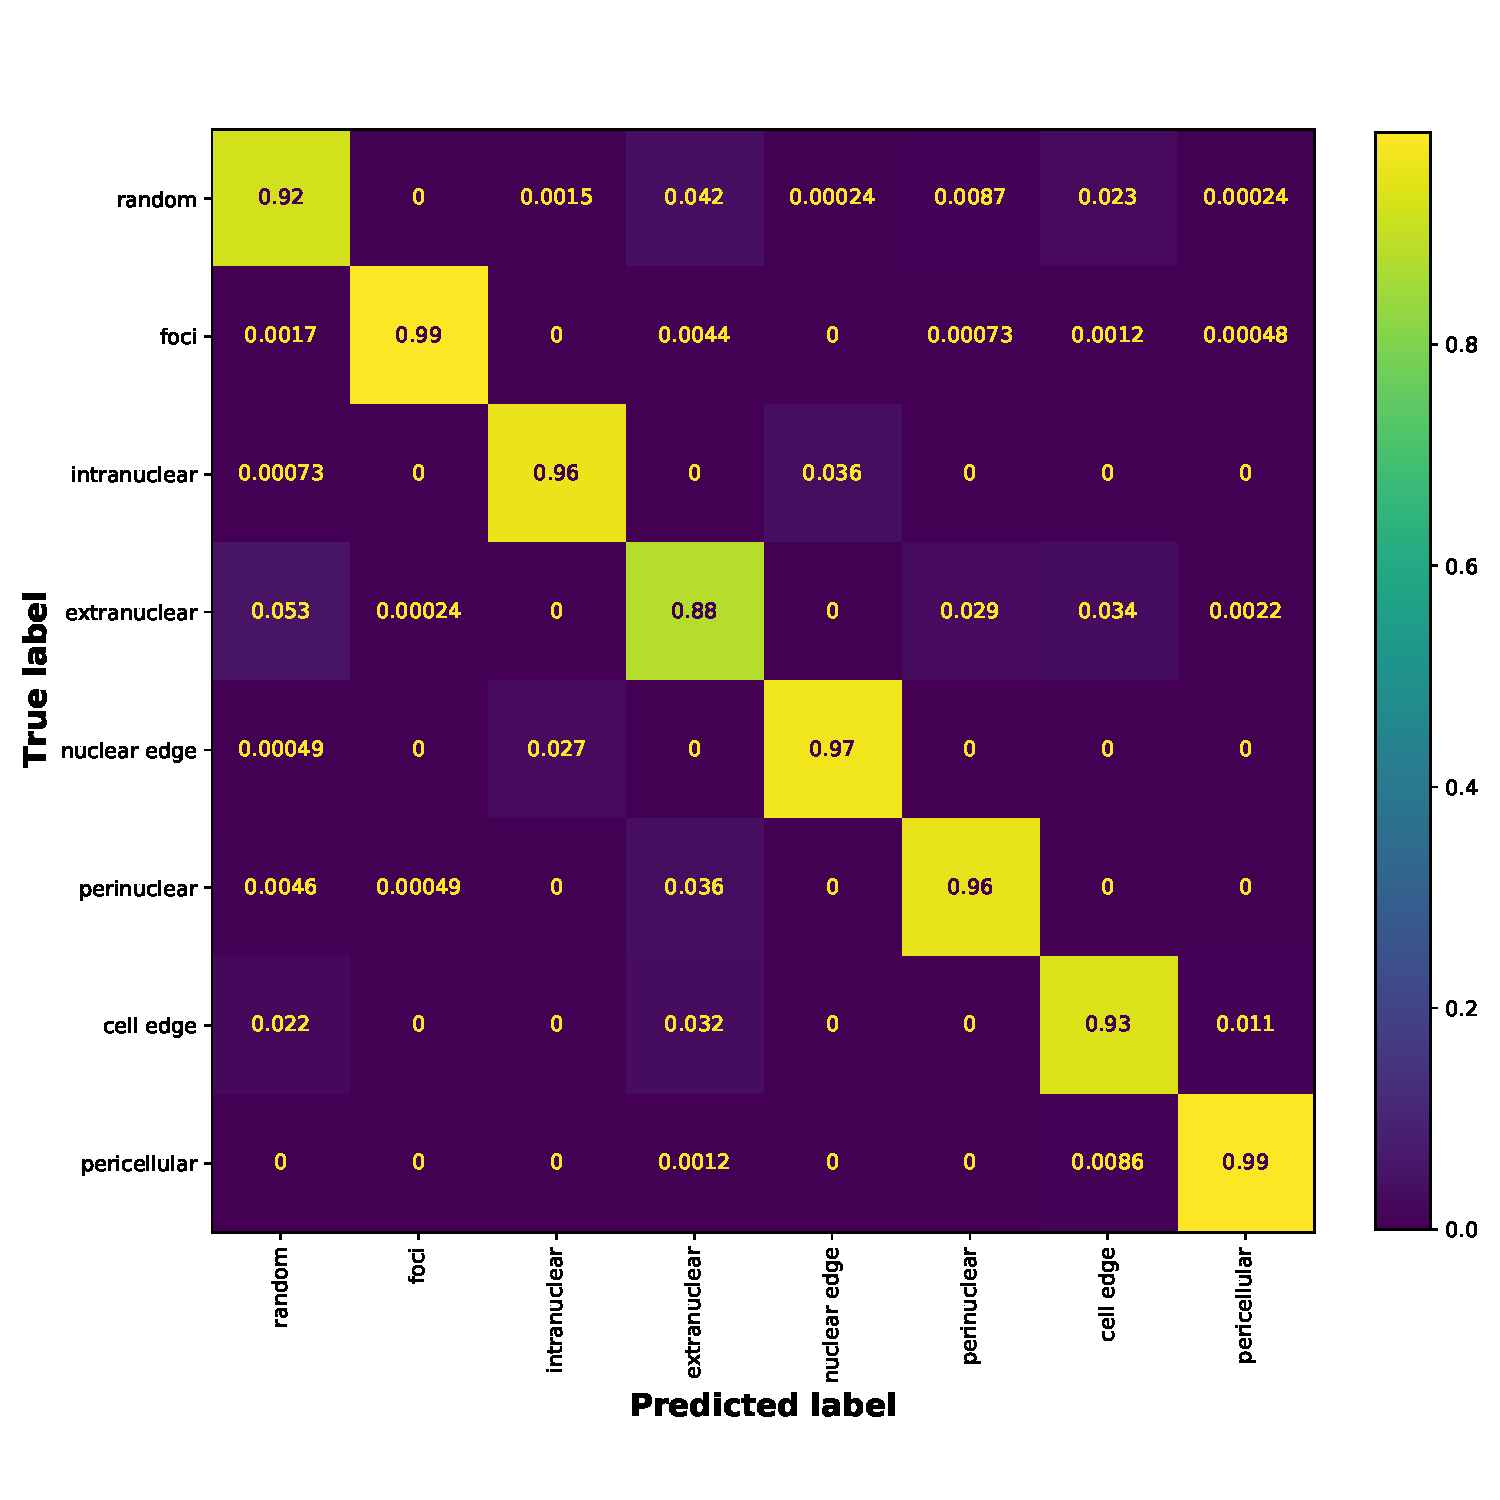
\includegraphics[width=0.7\textwidth]{figures/chapter4/confusion_matrix}
    \caption{Confusion matrix with simulated patterns}
    \label{fig:confusion_matrix}
\end{figure}


\subsection{Embedding extraction} \label{subsec:learned_embedding}

% brief description of the real dataset
% results supervised
% plot boxplot
% results unsupervised
% plot umap
% (plot dendogram)

\begin{figure}[h]
    \centering
    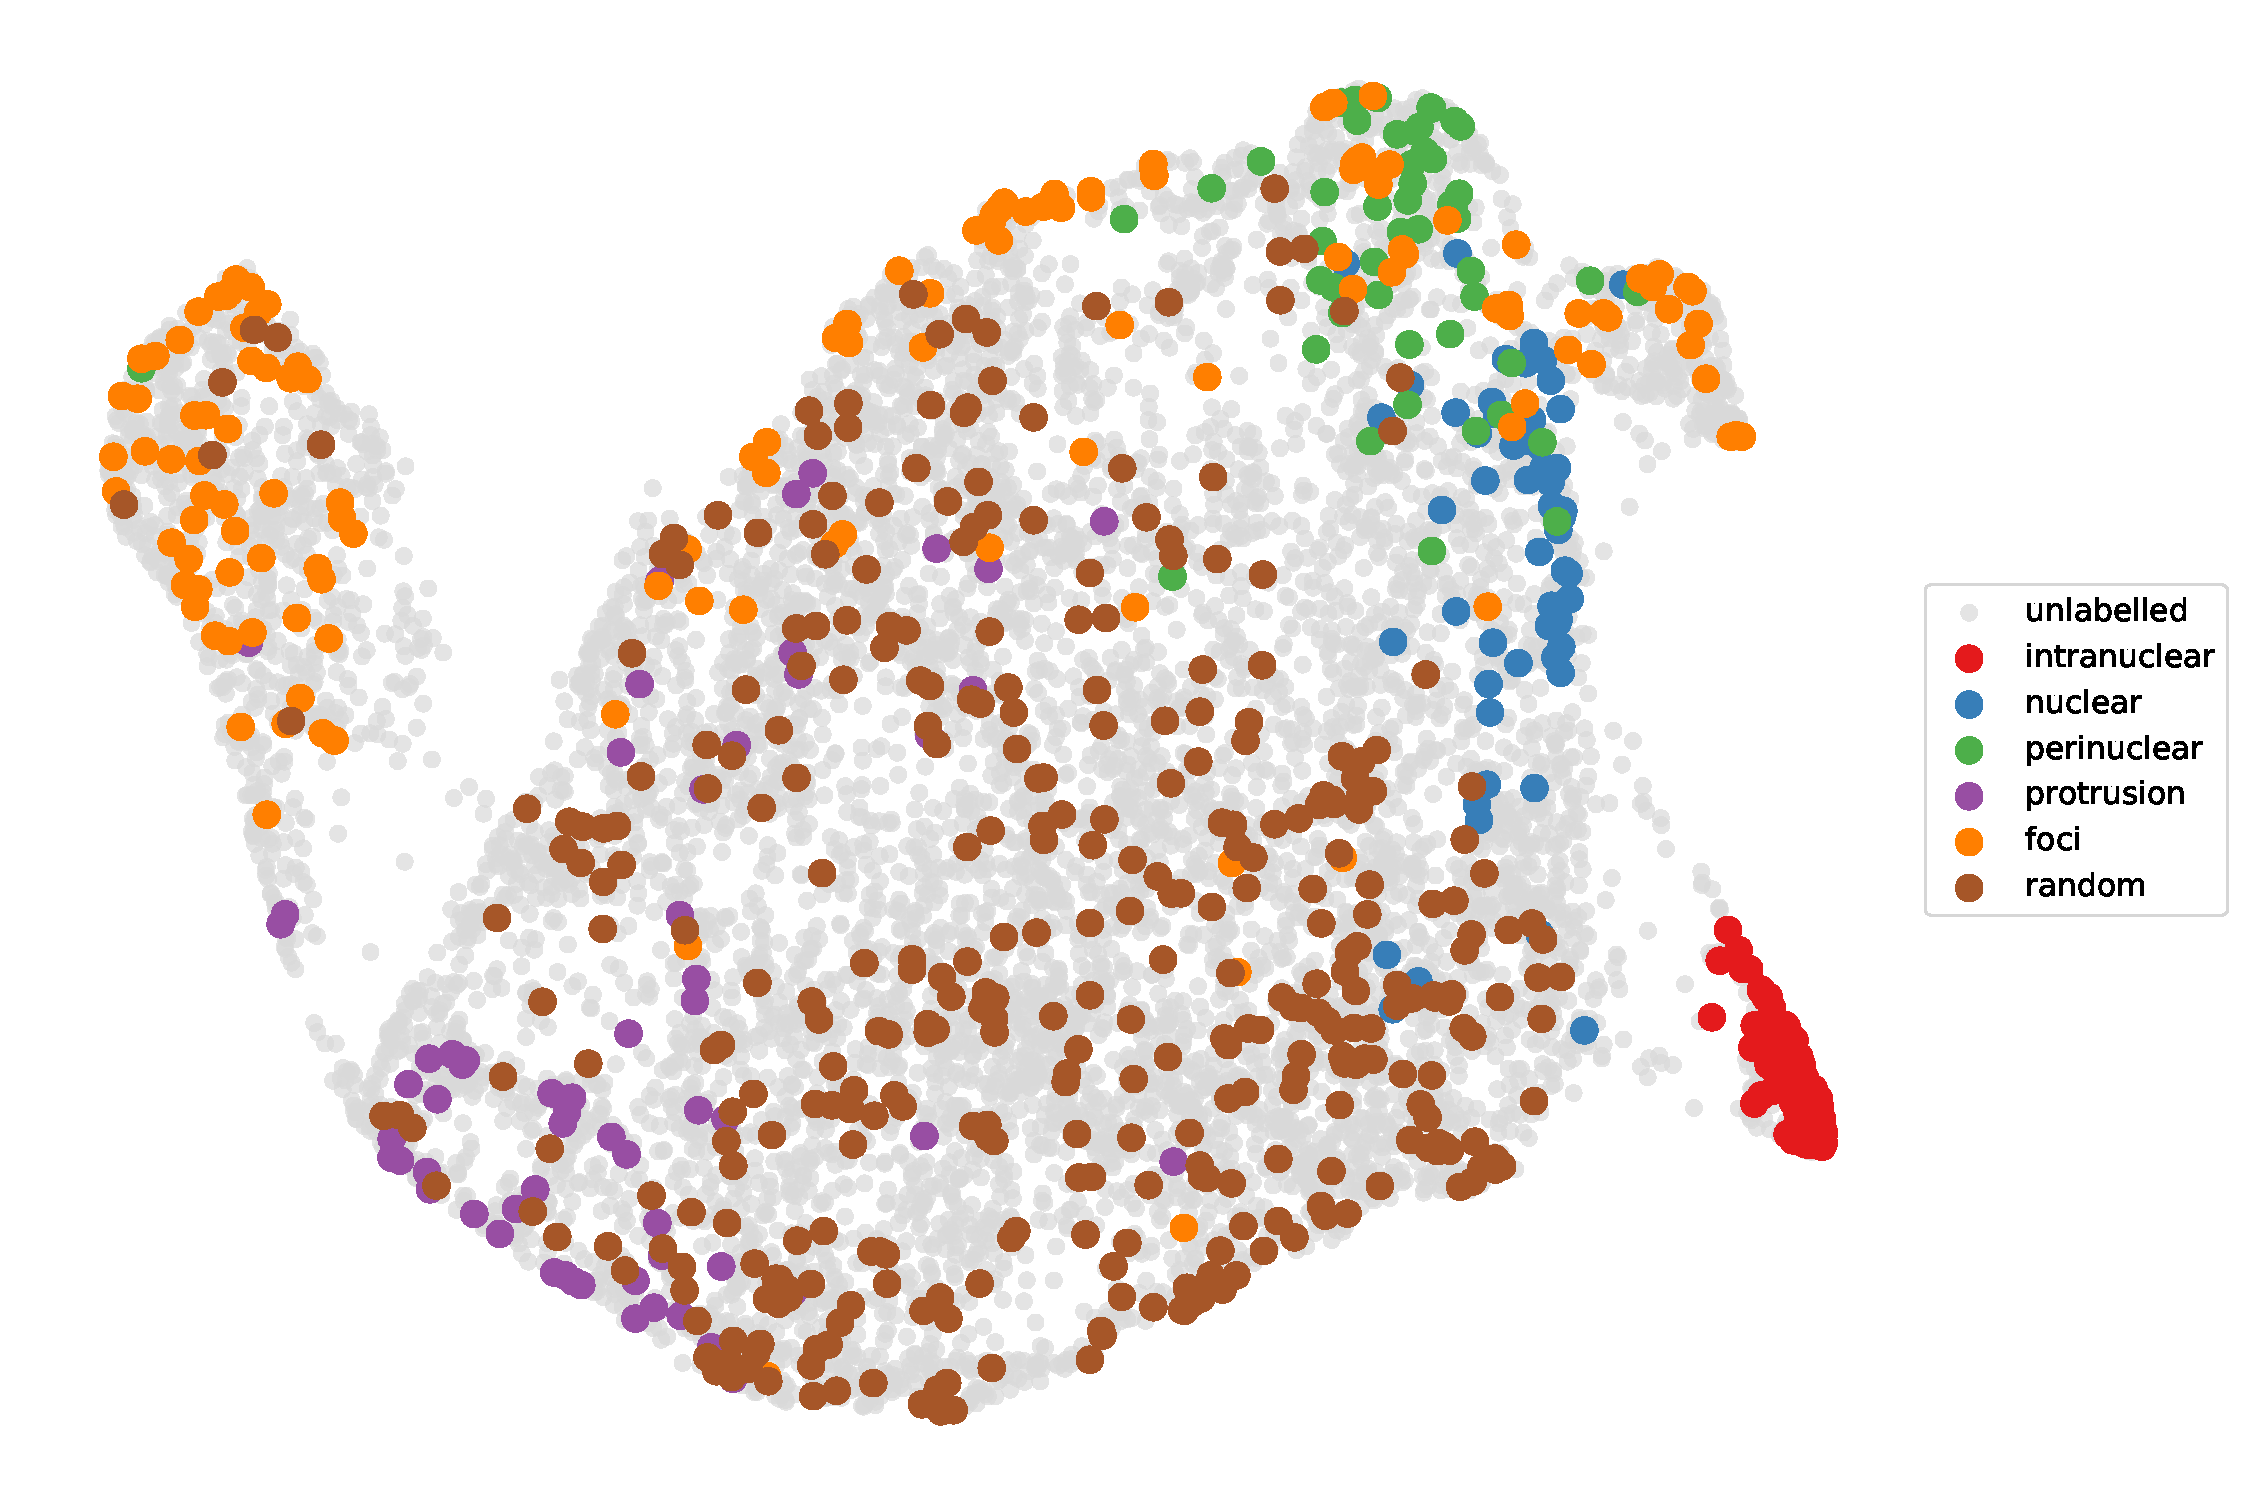
\includegraphics[width=1\textwidth]{figures/chapter4/umap_real}
    \caption{UMAP embedding with learned features}
    \label{fig:umap_real}
\end{figure}

\begin{figure}[h]
    \centering
    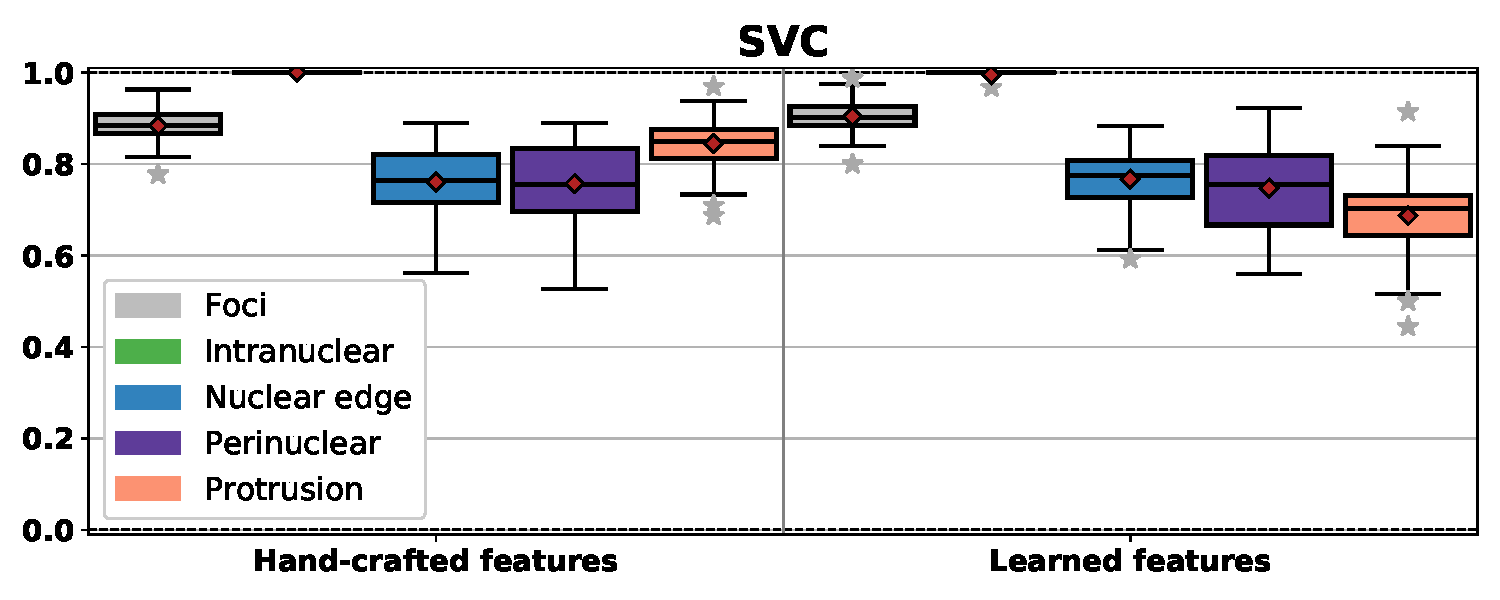
\includegraphics[width=1\textwidth]{figures/chapter4/f1_SVC}
    \caption{F1-score with localization pattern classification (SVC model)}
    \label{fig:f1_SVC_real}
\end{figure}


\section{Conclusion} \label{sec:analysis_conclusion}

% learned features from convnet
% from features engineering to simulation engineering